\documentclass{article}

\usepackage[a4paper, total={7in, 9in}]{geometry}
\pagestyle{empty} % Prevent relative page numbers

%%%%%%%%%%%%%%%%%%%%%%%%%%%%%%%%%%%%%%
%% Default definitions 
%% Define listings format
\usepackage{xcolor} % Required for listings color definitions
\definecolor{Brown}{cmyk}{0,0.81,1,0.60}
\definecolor{OliveGreen}{cmyk}{0.64,0,0.95,0.40}
\definecolor{CadetBlue}{cmyk}{0.62,0.57,0.23,0}
\definecolor{lightlightgray}{gray}{0.9}

\usepackage{listings} % computer code language formatting

\lstdefinestyle{tex-style} {
	language=[LaTeX]TeX,                    % Code langugage
	basicstyle=\ttfamily,                   % Code font, Examples: \footnotesize, \ttfamily
	%keywordstyle=\color{OliveGreen},        % Keywords font ('*' = uppercase)
	commentstyle=\color{gray},              % Comments font
	numbers=none,                           % Line nums position
	numberstyle=\tiny,                      % Line-numbers fonts
	stepnumber=1,                           % Step between two line-numbers
	numbersep=5pt,                          % How far are line-numbers from code
	backgroundcolor=\color{lightlightgray}, % Choose background color
	frame=single,                             % A frame around the code
	tabsize=2,                              % Default tab size
	captionpos=b,                           % Caption-position = bottom
	breaklines=true,                        % Automatic line breaking?
	breakatwhitespace=false,                % Automatic breaks only at whitespace?
	showspaces=false,                       % Dont make spaces visible
	showtabs=false,                         % Dont make tabls visible
	columns=flexible,                       % Column format
	morekeywords={__global__, __device__}  % CUDA specific keywords
}
\lstnewenvironment{latex}
{\lstset{language=[LaTeX]TeX}}
{}
\lstset{style=tex-style}

%% Define URL format
\usepackage[hyphens]{url}
\usepackage{hyperref}
\hypersetup{
	colorlinks=true,
	citecolor=black,
	filecolor=black,
	linkcolor=blue,
	urlcolor=blue
}

\setlength\parindent{0pt}


%%%%%%%%%%%%%%%%%%%%%%%%%%%%%%%%%%%%%%
%% Example-specific packages
\usepackage{pgfplots}
\usetikzlibrary{arrows}

%%%%%%%%%%%%%%%%%%%%%%%%%%%%%%%%%%%%%%
%% Example-specific preamble
\pgfplotsset{width=8cm, compat=1.13}

\begin{document}

\section*{Dual axes in tikz}

\subsection*{Description}
Dual scaling in a tikz figure is a common need. This example shows a nice way to have two y axes in a single tikzpicture; one on the left and one on the right.

\subsection*{Sources}
\url{https://tex.stackexchange.com/questions/316978/how-to-draw-a-graph-with-several-axes?newsletter=1&nlcode=544695%7c921f}

\subsection*{Used Packages}
\verb|pgfplots|

\subsection*{Preamble}
\begin{latex}
%%%%%%%%%%%%%%%%%%%%%%%%%%%%%%%%%%%%%%
%% Example-specific packages
\usepackage{pgfplots}
\usetikzlibrary{arrows}

%%%%%%%%%%%%%%%%%%%%%%%%%%%%%%%%%%%%%%
%% Example-specific preamble
\pgfplotsset{width=8cm, compat=1.13}
\end{latex}

\subsection*{Document}
\begin{latex}
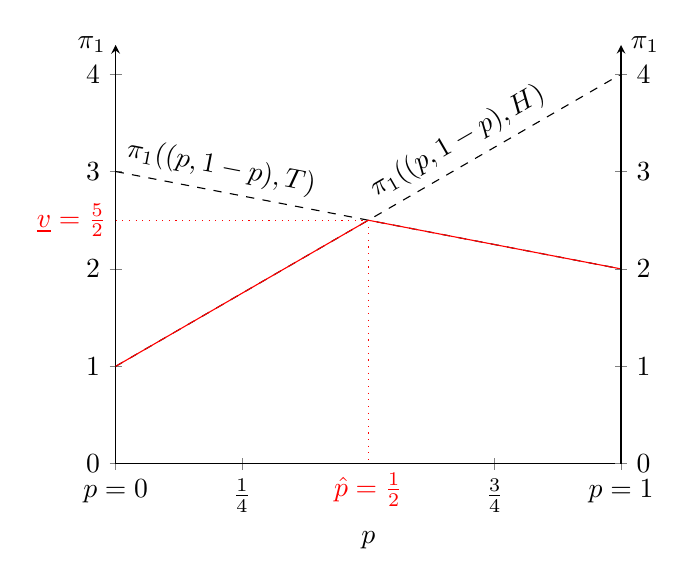
\begin{tikzpicture}
\pgfplotsset{% <-- common presets for both axes
	ylabel=$\pi_1$,
	domain=0:1,xmin=0,xmax=1,
	ymin=0,ymax=4.3,
	enlargelimits=false,
	clip=false % Controls whether any paths inside of an axis shall be clipped. Used to avoid clipping red text which is outside the plot limits.
}
\begin{axis}[
axis y line=left,                   % <-- left y axis
ylabel style={at={(0,1)},rotate=-90,anchor=east},% <--
axis x line=bottom,                 % <--
x axis line style={-},              % <--
xlabel=$p$,
xtick={0, 0.25, 0.75, 1},           % <--
xticklabels={$p=0$, $\frac{1}{4}$, $\frac{3}{4}$, $p=1$},% <--
]
\addplot[dashed] { -x+3} node[above,sloped,pos=0.2] {$\pi_1((p,1-p),T)$};
\addplot[dashed] {3*x+1} node[above,sloped,pos=0.7] {$\pi_1((p,1-p),H)$};
\addplot[red] {ifthenelse(x>0.5,-x+3,3*x+1)};
\draw[dotted,red] (0,5/2) node[left] {$\underline{v} = \frac{5}{2}$}
-| (0.5,0) node[below] {$\hat{p} = \frac{1}{2}$}; % path elements (i.e. the nodes) are outside of the graph area
\end{axis}
%
\begin{axis}[
axis y line=right,                  % <-- right y axis
ylabel style={at={(1,1)},rotate=-90,anchor=west},% <--
axis x line=none,                   % <-- Disable second x axis to avoid overlap
]
\end{axis}
\end{tikzpicture}
\end{latex}

\subsection*{Result}

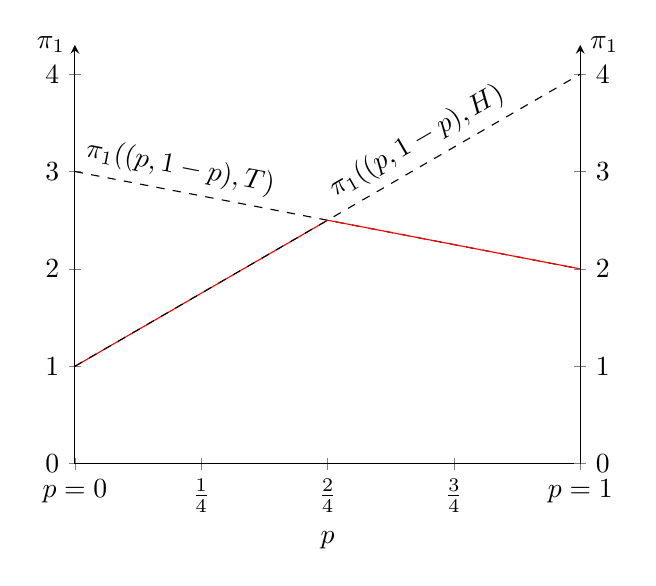
\begin{tikzpicture}
\pgfplotsset{% <-- common presets for both axes
	ylabel=$\pi_1$,
	domain=0:1,xmin=0,xmax=1,
	ymin=0,ymax=4.3,
	enlargelimits=false,
}
\begin{axis}[
axis y line=left,                   % <-- left y axis
ylabel style={at={(0,1)},rotate=-90,anchor=east},% <--
axis x line=bottom,                 % <--
x axis line style={-},              % <--
xlabel=$p$,
xtick={0, 0.25, 0.5, 0.75, 1},           % <--
xticklabels={$p=0$, $\frac{1}{4}$, $\frac{2}{4}$, $\frac{3}{4}$, $p=1$},% <--
]
\addplot[dashed] { -x+3} node[above,sloped,pos=0.2] {$\pi_1((p,1-p),T)$};
\addplot[red] {ifthenelse(x>0.5,-x+3,3*x+1)};
\end{axis}
%
\begin{axis}[
axis y line=right,                  % <-- right y axis
ylabel style={at={(1,1)},rotate=-90,anchor=west},% <--
axis x line=none,                   % <-- Disable second x axis to avoid overlap
]
\addplot[dashed] {3*x+1} node[above,sloped,pos=0.7] {$\pi_1((p,1-p),H)$};
\end{axis}
\end{tikzpicture}

\end{document}